\subsection{Systemarchitektur}

\subsubsection{Contiki}
Contiki ist ein Open Source Echtzeitbetriebssystem, das bei uns in der PG auf den MICAz-Modulen eingesetzt wird.
Contiki bietet einen einfachen ereignisgesteuerten Betriebssystemkern mit sogenannten Protothreads, optionalem 
pr\"aemptiven Multiprogramming, Interprozesskommunikation via Messagepassing durch Events, eine dynamische Prozessstruktur
mit Unterst\"utzung f\"ur das Laden und Entladen von Programmen, nativen TCP/IP-Support über den uIP TCP/IP-Stack und eine 
grafische Benutzerschnittstelle, welche direkt auf einem Bildschirm oder als virtuelle Anzeige \"uber Telnet oder VNC genutzt werden kann \cite{Wikipedia:2013:Online}.
 
\paragraph{Systemarchitektur}
Ein laufendes Contiki System besteht aus dem Kernel, Bibliotheken, Prozessen und dem Programm-Lader, mit dem Anwendungen zur Laufzeit aus dem Speicher oder \"uber ein Funkmodul geladen werden k\"onnen.
Die unten stehende Abbildung zeigt die Aufteilung des Betriebssystems in zwei Teile. 
\begin{figure}[h!]
	\centering
		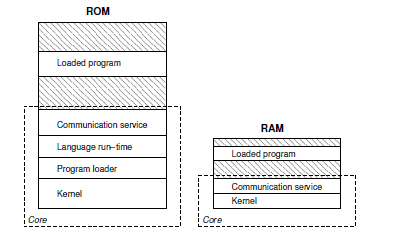
\includegraphics[width=0.9\textwidth]{Systemarchitektur_Contiki.png}
	\caption{Komponenten von Contiki \cite{Dunkels:Groenvall:Voigt:2014:Online}}
	\label{Systemarchitektur von Contiki}
\end{figure}
Der Core ist ein Basissystem und besteht aus dem Kernel, Bibliotheken, Ger\"{a}tetreibern und dem Programm-Lader. 
Im allgemeinen sind \"Anderungen am Core nicht vorgesehen und nur unter Verwendung eines speziellen Bootloaders m\"oglich. 
Die konkrete Aufteilung des Systems in Core und ladbare Programme wird beim Kompilieren des Systems entschieden und h\"angt 
von der Hardware-Plattform ab \cite[vgl.][S. 7]{Walter:2010}. Ger\"atetreiber werden als Bibliotheken implementiert. 

\paragraph{Events}
In Contiki kommunizieren Prozesse \"uber Events. Auch der Kernel versendet Events, um Prozesse \"uber ihren Status 
(Init, Continue, Exit) oder \"uber abgelaufene Timer zu Informieren. Zur Identifikation stehen dabei Event IDs zur 
Verf\"ugung. Die Event IDs 0-127 k\"onnen vom Benutzer frei vergeben werden, w\"ahrend die Prozess IDs ab 128 vom 
System genutzt werden. Grunds\"atzlich unterscheidet Contiki zwischen synchronen und asynchronen Events. 
\begin{itemize}
\item \textbf{Asynchrone Events} sind eine Form der Deferred Procedure Call: asynchrone Events werden vom Kernel in einer 
Warteschlange gespeichert. Die Scheduling-Funktion des Kernels l\"auft nach Systemstart in einer Endlosschleife. 
In jedem Durchlauf wird ein Event aus der Schlange entnommen und wird einige Zeit sp\"ater an den Zielprozess weitergeleitet.
\item \textbf{Synchrone Events} gleichen einem Funktionsaufruf.
Sie werden ohne Umweg \"uber die Warteschlange direkt an den Empf\"anger-Prozess
zugestellt \cite[vgl.][S. 7]{Walter:2010}.  Mit der Funktion process\_post\_synch(\&example\_process, EVENT\_ID, msg) wird gezielt ein 
Prozess aufgerufen (ein Broadcast ist nicht m\"oglich). W\"ahrend der aufgerufene Prozess aktiv ist, blockiert der Aufrufer und 
setzt seine Ausführung erst fort, wenn der aufgerufene Prozess die Kontrolle wieder abgibt.
\end{itemize}

\paragraph{Prozesse}
Prozesse in Contiki implementieren ein Konzept namens Protothreads. Dies erlaubt es Prozessen, ohne den Overhead und die langen 
Prozesswechselzeiten von normalen Threads auszukommen. Gleichzeitig k\"onnen trotzdem andere Prozesse ausgef\"uhrt werden, falls ein Prozess auf ein Event (Timer, Nachricht von anderem Prozess...) warten muss.
F\"ur die Entwicklung mit Prozessen ist wichtig, dass nicht-statische Variablen nicht zwischen zwei Aufrufen erhalten bleiben.
Der relevante Status eines Prozesses sollte daher mithilfe von statischen Variablen abgelegt werden (siehe Variable i im folgenden Beispiel)

\begin{figure}[h!]
	\centering
		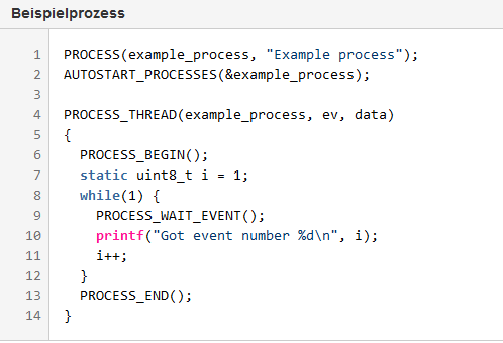
\includegraphics[width=0.9\textwidth]{Beispielprozess.png}
	\label{Beispielprozess}
\end{figure}
In Zeile 1 wird der Prozess initialisiert und in Zeile 2 automatisch beim Boot von Contiki gestartet. Zeile 4 beinhaltet die
Deklaration. So k\"onnen andere Prozesse diesem Prozess Events (mit oder ohne Daten) schicken, auf die unser Beispielprozess 
mit ev und data zugreifen kann. Zeile 6 kennzeichnet den Beginn der tats\"achlichen Ablauflogik. Code \"uber dieser Zeile wird 
bei jedem Prozessaufruf ausgef\"uhrt, dies wird jedoch in den meisten F\"allen nicht ben\"otigt. Zeile 13 schlie{\ss}lich beendet
den Prozess und entfernt ihn aus der Prozess-Liste des Kernels. In diesem Beispiel wird die Zeile jedoch nie erreicht, sodass der Prozess immer wieder aufgerufen wird, bis er von einem anderen Prozess beendet wird.
Wichtige Funktionen in Prozessen:
\begin{itemize}
\item PROCESS\_WAIT\_EVENT() - Wartet auf ein beliebiges Event, bevor die Ausf\"{u}hrung fortgesetzt wird.
\item PROCESS\_WAIT\_EVENT\_UNTIL(condition) - Wartet auf ein beliebiges Event, setzt die Ausf\"{u}hrung aber nur fort, wenn die Bedingung erf\"{u}llt ist.
\item PROCESS\_WAIT\_UNTIL() - Wartet, bis die Bedingung erf\"ullt ist. Muss den Prozess nicht zwangsl\"{a}ufig anhalten.
\end{itemize}
Prozesse k\"onnen \"uber Events (siehe Events) oder Polling-Anfragen kommunizieren.  Polls sind Events mit hoher Priorit\"at und 
k\"onnen genutzt werden, um den angerufenen Prozess so schnell wie m\"oglich auszuf\"uhren. Sie
sind besonders bei der Abarbeitung von Hardware-Interrupts wichtig, da Interrupts-Handler keine Events, sondern nur
Polling-Anfragen absetzten d\"urfen \cite[vgl.][S. 7]{Walter:2010}.

\subsubsection{Treiber, Services und Interfaces}
Auf dieser Ebene werden der Agenten RTE alle Funktionalitäten zur Verfügung gestellt. Das RTOS stellt Infrastruktur wie z.~B. Task Management, Timing, Events usw.
Die Driver Ebene kümmert sich um die Schnittstellen/Pins des Controllers wie z.~B. Protokolle angeschlossener
Devices\cite[S. 26]{Stasch:Hahn}. Die Aufgabe des Service ist es, Funktionen für spezielle Anwendungen zur Verfügung zu stellen.
Darüber kommen die Interfaces. Diese sind nötig, damit bestimmte Funktionen immer gleich der Agenten RTE zur Verfügung gestellt werden, auch wenn der Service anders ist oder wenn ein Service verschiedene Interfaces bedienen soll\cite[S. 26]{Stasch:Hahn}.

\subsubsection{Agenten RTE}
\label{sec:AgentRTE}
Auf der nächsten Hierarchieebene über den Interfaces liegt die Laufzeitumgebung der Agenten (AgentRTE). Es ist die erste plattformunabhängige Ebene über den Interfaces und dem Betriebssystem. Vergleicht man die Implementation für STASH-Controller und \textsc{Mica}z-Module, unterscheidet sich das AgentenRTE lediglich im Prozessmodell der Agenten, das abhängig vom Betriebssystem ist: Während die STASH-Controller mit dem MSP430-Mikrocontroller auf SYS/BIOS mit präemptivem Scheduling stetzen, läuft auf den \textsc{Mica}z-Modulen ein nicht-präemptives Contiki-System. Die Agenten auf den Stash-Controllern werden daher jeweils durch einen eigenen Prozess repräsentiert, während es auf den \textsc{Mica}z-Modulen einen gemeinsamen Prozess gibt, der Agenten über Funktionszeiger aufruft. Wir gehen hier nur auf die Implementierung auf den \textsc{Mica}z-Modulen ein.

Neben dem Aufruf der einzelnen Agenten ist das AgentenRTE auch für das Registrieren und Terminieren der Agenten und den Austausch beziehungsweise die Verteilung von Nachrichten verantwortlich.

\paragraph{Verwaltung der Agenten}\mbox{}\\
Agenten werden mit ID und Typ registriert. Nach Konvention bekommt dabei der Plattform-Agent stets die ID des Moduls, der Order-Agent eine um eins erhöhte ID und der Routing-Agent eine um zwei erhöhte ID. Hat Beispielsweise das Modul die ID \textit{0x0110}, so hat der Plattform-Agent ebenfalls die ID \textit{0x0110}, der Order-Agent die ID \textit{0x0111} und der Routing-Agent schließlich die ID \textit{0x0112}. Die Registrierung dieser Agenten erfolgt in der Main-Methode des Systems. Die Nummerierung der Paket-Agenten ist unabhängig von dieser Konvention, allerdings muss darauf geachtet werden, dass ihre IDs nicht mit den übrigen Agenten übereinstimmen.

Registrierte Agenten werden in ein Array aus Agenten-Strukturen eingetragen und dort verwaltet.
\autoref{lst:agentstruct} zeigt die Agenten- und Agenten-Callback-Strukturen. Außerdem wird einmalig ihre Init-Methode aufgerufen.

Bei der Ausführung wird nun bei jedem Prozessaufruf des Agenten-Prozesses eine Zählervariable erhöht, die jeweils die Main-Methode des nächsten Agenten aufruft. Da  Contiki ein nicht-präemptives Scheduling nutzt, dürfen die Agenten nicht blockieren, sondern müssen die Kontrolle an den Haupt-Prozess zurückgeben, sprich die Main-Methode muss terminieren.

\lstinputlisting[language=C, style=customc, captionpos=b, caption={Agenten Strukturen in C}, label=lst:agentstruct]{src/flow/lst/agent_struct.lst}

\paragraph{Austausch von Nachrichten}\mbox{}\\
Der Austausch von Nachrichten und damit die Kommunikaion zwischen Agenten ist unerlässlich in einem Multiagentensystem. Auch diese Aufgabe kommt dem AgentenRTE zu. Die Laufzeitumgebung prüft den Empfänger einer Nachricht und übergibt sie schließlich an den richtigen Agenten. Der Aufbau einer solchen Agenten-Nachricht wird durch eine Struktur beschrieben, die in \autoref{lst:commsg} abgebildet ist. Der Kopf einer Nachricht ist demnach 15 Byte groß, die Nutzdaten können bis zu 26 Byte betragen.

\lstinputlisting[language=C, style=customc, captionpos=b, caption={Struktur einer Agenten-Nachricht in C}, label=lst:commsg]{src/flow/lst/message_struct.lst}

Sendet ein Agent eine solche Nachricht, übergibt er sie dem AgentRTE. Dieses prüft, ob sich der Empfänger-Agent auf dem eigenen Modul befindet. Ist das der Fall, wird die Nachricht in der Warteschlange für eingehende Nachrichten gespeichert und kann dort vom Empfänger abgerufen werden. Wenn der Agent nicht auf der Plattform registriert ist, wird die Nachricht an das CommunicationInterface weitergeleitet, das sich zum die Verteilung im Netzwerk kümmert. So gelangt die Nachricht auch über die Modulgrenzen hinweg zum richtigen Agenten.

Eingehende Nachrichten werden vom CommunicationInterface an das AgentRTE weitergereicht. Dafür wird zunächst angefragt, ob sich der Ziel-Agent beziehungsweise einer der Ziel-Agenten im Falle von Gruppennachrichten auf der Plattform befindet. Ist dies der Fall wird die Nachricht in der Warteschlange für eingehende Nachrichten gespeichert.

Ein großes Problem bei Nachrichtenaustausch stellt der mit 4 KB sehr begrenzte Arbeitsspeicher der \textsc{Mica}z-Module dar. Entsprechend ist der Platz in der Warteschlange für eingehende Nachrichten begrenzt, pro Agent können nur drei Nachrichten gespeichert werden. Um den Speicher nicht überlaufen zu lassen und dadurch Nachrichten zu verlieren, wird daher das Senden von Nachrichten durch ein Token-System begrenzt. Pro Agent kann so in jedem Durchlauf nur eine Nachricht versendet werden. Nutzt ein Agent dies nicht aus, kann sein Token auf einen anderen Agenten übertragen werden. In der Praxis schränkt diese Restriktion die Agenten in ihrer Funktionalität jedoch nicht ein. Meist erfordert eine eingehende Nachricht nur eine direkt Antwort oder die Benachrichtigung eines anderen Agenten. Müssen einmal doch zwei oder mehr Nachrichten als Reaktion versendet werden, geschieht dies mithilfe von Zwischenzuständen und Flags, die beim nächsten Durchlauf aktiv werden.
%\begin{figure}[h!]
%	\centering
%		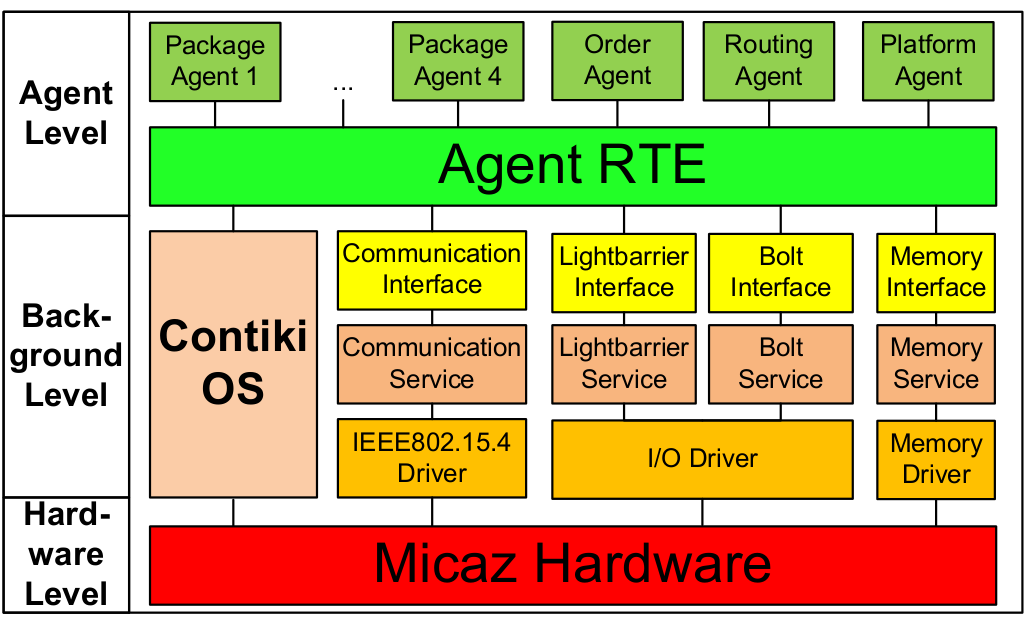
\includegraphics[width=0.9\textwidth]{ArchitekturMicazRampe.png}
%	\caption{Architektur Micaz Rampe\cite{Stasch:Hahn}}
%	\label{ArchitekturMicazRampe}
%\end{figure}

\subsection{Agenten}
Oberhalb des AgentRTE sind die Agenten implementiert. Sie bilden die oberste Ebene des Systems und implementieren die eigentliche Funktionalität. Dabei greifen sie auf das AgentenRTE und die verschiedenen Interfaces zu und kommunizieren untereinander über Agenten-Nachrichten. Auf jedem Modul agieren ein Plattform-Agent, der die Sensoren und Aktoren der Plattform steuert, ein Order-Agent, der zusammen mit anderen Order-Agenten die Betriebslogik des Materialflusssystems darstellt, ein Routing-Agent, der gemeinsam mit anderen Routing-Agenten die Pakete durch das System leitet und eventuell bis zu vier Paket-Agenten, die die physischen Pakete repräsentieren und durch das System wandern. Die einzelnen Agenten sind im Folgenden beschrieben.
\subsubsection{Paket-Agent}
Ein Paket Agent repräsentiert ein physisches Paket. Seine ID ist gleichzeitig auch Paketnummer. Beim Eintritt im System wird vom Plattform-Agent ein neuer Paket-Agent initialisiert. Wechselt ein Paket von einem Modul auf das nächste, so wandert auch der Paket-Agent auf das neue Modul. Dies wird erreicht, indem der Agent auf dem einen Modul beendet und auf dem nächsten mit seinem Ziel und seiner ID neu initialisiert wird. Dies ist möglich, da sich verschiedene Pakete nur durch ihr Ziel und ihre ID voneinander unterscheiden. Die Übertragung der Paket-Agenten wird von den Plattform-Agenten der jeweiligen Module übernommen.

Das Ziel von Paket-Agenten ist dynamisch. Es wird von den Order-Agenten verwaltet. Kommt ein neuer Auftrag ins System, wird vom Order-Agenten, der den Auftrag verwaltet, eine Nachricht an das entsprechende Paket gesendet. Erhält der Paket-Agent eine solchen Nachricht, wird dem Order-Agenten der Empfang bestätigt und das eigene Ziel wird angepasst.

Hat der Paket-Agent ein gültiges Ziel und wird ihm vom Plattform-Agenten per Flag die Erlaubnis erteilt, sendet er dem Routing-Agenten seiner Plattform eine Routing-Anfrage, bestehend aus dem Ziel des Pakets. Wenn diese nicht abgelehnt wird, wartet der Paket-Agent, bis sein Ziel geändert wird, oder sich auf einer Plattform befindet, die nicht seinem aktuellen Ziel entspricht und er die erneute Erlaubnis bekommt, eine Routing-Anfrage zu stellen. Wird die Anfrage dagegen abgelehnt, stellt er beim nächsten Aufruf eine neue, bis die Anfrage vom Routing-Agenten angenommen wird.

Schließlich kann der momentane Zustand des Pakets über eine sogenannte \textit{UPDATE\_PHYSICAL}-Nachricht von einem Gateway abgefragt werden. Der Agent antwortet darauf mit der ID der Plattform, auf der er sich zur Zeit befindet und dem eigenen Ziel.
\subsubsection{Plattform-Agent}
Der Plattform-Agent ist der einzige plattformabhängige Agent des Systems. Während alle anderen Agenten auf allen Modultypen identisch sind, ist der Plattform-Agent modulspezifisch. Seine Aufgabe ist die Steuerung und Überwachung seines Moduls.

Beiden gemeinsam ist jedoch die Übertragung, also das Beenden und die erneute Initialisierung, von Paket-Agenten. Diese wird immer vom Volksbot initialisiert. Es wird eine Anfrage an den Plattform-Agenten der jeweiligen Rampe gesendet, entweder nach einem Lagerplatz oder nach einem speziellen Paket, abhängig davon, ob ein Paket abgelegt oder aufgenommen werden soll. Soll ein Paket abgelegt werden, muss die Anfrage bestätigt werden, bevor ein Registrierungs-Auftrag mit den Details des Paket-Agenten gesendet wird und der Agent auf seiner momentanen Plattform terminiert wird. Soll ein Paket aufgenommen werden, prüft die Rampe, ob das Paket mit der geforderten ID vorhanden ist und ausgegeben werden kann und sendet im Erfolgsfall ebenfalls einen Registrierungs-Auftrag und terminiert seinerseits den  entsprechenden Paket-Agenten, der dann auf dem Volksbot neu initialisiert wird.

Außerdem geben beide auf eine \textit{UPDATE\_PHYSICAL}-Nachricht die IDs aller Paket-Agenten zurück, die sich derzeit auf dem Modul befinden.

Im Folgenden werden nun die plattformspezifischen Eigenschaften der Plattform-Agenten beschrieben.

\paragraph{Plattform-Agent der Rampen}\mbox{}\\
Der Plattform-Agent auf einer Rampe ist neben der Verwaltung der Paket-Agenten auch für die Steuerung und das Auslesen der Bolzen über das Bolt\_Interface beziehungsweise Lichtschranken über das Photosensor\_Interface verantwortlich. Er sorgt dafür, dass die Pakete korrekt vereinzelt werden und verwaltet ihre Reihenfolge. Außerdem prüft er auf die Anfrage eines Volksbots, ein Paket abzulegen, anhand der Lichtschranken, ob noch ein Platz auf der Rampe zur Verfügung steht.
\paragraph{Plattform-Agent der Volksbots}\mbox{}\\
Der Plattform-Agent auf einem Volksbot kommuniziert mit dem Laptop, der den Volksbot steuert. Er erhält eine Nachricht, wenn der Volksbot seine Ziel-Position erreicht hat. Daraufhin initiiert er die Übergabe des Paketes. War die Übergabe des Paket-Agenten erfolgreich, sendet der dem Laptop eine Nachricht über die serielle UART-Nachricht um das Fließband auf dem Volksbot zu starten und die physische Übernahme des Pakets zu starten.
\subsubsection{Order-Agent}
Die Order-Agent übernehmen die Rolle eines zentralen Materialflussrechner im Materialflusssystem. Ihre Aufgabe ist die Verarbeitung von Aufträgen, sprich die Zuweisung von Zielen an Pakete. Aufträge bestehen aus Paket- und Ziel-ID und werden über ein Gateway in das System eingegeben. Dafür wird eine entsprechende Agenten-Nachricht an einen einzelnen Order-Agenten gesendet, der den Empfang bestätigt oder ablehnt, falls kein Platz in seinem Speicher zur Verfügung stand. In diesem Fall muss ein anderer Order-Agent mit dem Auftrag betraut werden. Ein Auftrag wird mit seiner Paket- und Ziel-ID sowie einem Status ("zu bearbeiten" beziehungsweise "in Verteilung") in einer Warteschlange ablegt.

Hat der Order-Agent in einem Aufruf keine Nachricht erhalten, durchsucht er diese Warteschlange nach zu bearbeitenden Aufträgen und sendet eine Nachricht an das entsprechende Paket, sein Ziel zu ändern. Wird der Empfang dieser Nachricht vom Paket bestätigt, wird der Auftrag gelöscht, von nun an ist das Paket für die Erreichung seines Ziels verantwortlich. Sind alle Aufträge in Verteilung muss davon ausgegangen werden, dass die entsprechenden Nachrichten nicht angekommen sind oder die Pakete noch nicht im System sind. Daher wird in diesem Fall der Status aller Aufträge zurückgesetzt und es wird erneut versucht, Nachrichten an die einzelnen Pakete zu senden.
\subsubsection{Routing-Agenten}

Die Routing-Agenten kümmern sich um die Wegplanung der Pakete im Materialflusssystem. Sie suchen nach einem Volksbot, der ein Paket mit möglichst günstig zu seinem Ziel bringen kann. Dafür führen sie untereinander eine Auktion durch, bei der ein Transportauftrag zu möglichst geringen Kosten an einen Volksbot vergeben wird. Ein Routing-Agent reagiert dabei auf die Routing-Anfrage eines Paket-Agenten. Ein Routing-Agent kann gleichzeitig nur an einer Auktion teilnehmen beziehungsweise diese initiieren. Hiermit wird verhindert, dass ein Routing-Agent gleichzeitig zwei Auktionen gewinnt und deshalb eine der Auktionen zurückgerollt und wiederholt werden muss.

Die Routing-Agenten werden als kommunizierende Zustandsautomaten implementiert. Zustandsübergänge können durch eingehende Nachrichten oder Timer ausgelöst werden. \autoref{fig:routing_agent_fsm} zeigt den zugrunde liegenden Automaten.

\begin{figure}[h!]
  \centering
    \includegraphics[width = 1.35\textwidth, angle=90]{flow/RoutingAgent_FSM.png}
    \caption{Zustandsautomat des Routing Agenten}
    \label{fig:routing_agent_fsm}
\end{figure}

Ein Routing-Agent startet stets in Zustand 0. In diesem Zustand wartet er auf eingehende Routing-Anfragen. Diese können entweder von Paketen auf der eigenen Plattform oder von anderen Routing-Agenten kommen. Sie unterscheiden sich im ersten Byte der Conversation-ID einer Agenten-Nachricht. Hier ist die Autkions-ID gespeichert, die für neue Routing-Anfragen von Paketen erst durch den Routing-Agenten bestimmt werden muss und daher auf 0 gesetzt ist. 

Bei Eingang einer Routing-Anfrage durch ein Paket wird eine neue Routing-Anfrage an alle Routing-Agenten versendet, ein Timer gestartet, der abläuft, wenn die Bearbeitungszeit  und in Zustand 3 übergegangen. Kommt die Anfrage von einem anderen Routing-Agenten prüft der Agent, ob das Ziel erreichbar ist. Für Module auf einem Volksbot ist dies immer wahr, für Module an Rampen immer falsch. Ist das Ziel erreichbar, wird eine UART-Nachricht an den Volksbot gesendet, der die Kosten der Fahrt vom anfragenden Routing-Agenten zum Ziel des Pakets berechnen soll. Anschließend geht der Automat in Zustand 1 über.

In Zustand 1 wartet der Agent auf die Antwort des Volksbots auf seine Kostenanfrage. Geht diese ein und sind die Kosten größer als null, bedeutet dies, das Ziel ist erreichbar. Der Agent sendet anschließend diese Kosten an den Initiator der Auktion und geht in Zustand 2 über, wo er auf die Antwort des Initiators wartet. Wird das Angebot bestätigt, wird der Volksbot beauftragt, sich zum Ausgang des Initiators zu bewegen und der Automat geht in Zustand 6 über. Wird die Anfrage abgelehnt, geht der Automat zurück in Zustand 0 und wartet auf neue Anfragen. In Zustand 6 wartet der Routing Agent auf eine Nachricht des Plattform-Agenten, der bestätigt, dass das Paket abgegeben wurde und neue Anfragen angenommen werden können.

In Zustand 3 wartet der Routing-Agent auf Angebote von anderen Routing-Agenten, nachdem er eine Routing-Anfrage für ein Paket auf der eigenen Plattform verschickt hat. Er speichert diese Angebote mit Absender-ID und Kosten. Läuft schließlich der Bearbeitungs-Timer ab, wird geprüft ob mindestens ein Angebot eingangen ist. Ist das der Fall, wird das beste Angebot bestimmt und der Agent geht in Zustand 4 über. Andernfalls wird ein neuer Timer gesetzt, bis die Anfrage wiederholt wird und der Agent geht in Zustand fünf. In Zustand 5 wartet der Agent auf den Ablauf des Timers, versendet die Routing-Anfrage erneut an alle Routing-Agenten und geht zurück in Zustand 3. Zustand 4 dagegen bleibt aktiv, bis alle Teilnehmer der Auktion benachrichtigt wurden. In jedem Aufruf des Agenten wird eine Nachricht mit Cancel oder Acknowledge an einen weiteren Teilnehmer der Auktion gesendet. Sind alle Teilnehmer benachrichtigt, geht der Agent zurück in Zustand 0 und wartet auf neue Anfragen.